\documentclass{article}

% Geometry and layout
\usepackage[margin=1.2in]{geometry}
\usepackage[skip=10pt plus1pt, indent=0em]{parskip}
\usepackage{multicol}
\usepackage{titlesec}
\usepackage{csquotes}

% Links and references
\usepackage{hyperref}

% Math and symbols
\usepackage{amsmath}
\usepackage{amssymb}
\usepackage{amsthm}

% Graphics
\usepackage{graphicx}
\usepackage{svg}
\usepackage{tikz}

% Code listings
\usepackage{listings}
\usepackage{color}
\definecolor{dkgreen}{rgb}{0,0.6,0}
\definecolor{gray}{rgb}{0.5,0.5,0.5}
\definecolor{mauve}{rgb}{0.58,0,0.82}

% Frames and boxes
\usepackage{mdframed}

% Theorems and remarks
\newtheorem*{remark}{Remark}

\newcommand{\drawaxesgrid}[2]{
    % Draw x and y axes with arrows
    \draw[thick,->] (0,0) -- (#1,0) node[anchor=west] {\scriptsize x};
    \draw[thick,->] (0,0) -- (0,#2) node[anchor=north] {\scriptsize y};

    % Calculate the number of ticks based on sizes
    \pgfmathtruncatemacro{\xtickstop}{#1-1}
    \pgfmathtruncatemacro{\ytickstop}{#2-1}

    % a point at the origin (0, 0) 
    \filldraw [black] (0, 0) circle (5pt) {};

    % Draw x-axis tick marks and labels
    \foreach \x in {1,...,\xtickstop}
    \draw (\x,0.1) -- (\x,-0.1) node[anchor=south] {\scriptsize \x};

    % Draw y-axis tick marks and labels
    \foreach \y in {1,...,\ytickstop}
    \draw (0.1,\y) -- (-0.1,\y) node[anchor=east] {\scriptsize \y};

    % Draw light gray grid lines
    \foreach \x in {1,...,\xtickstop}
    \draw[lightgray,dashed] (\x,0) -- (\x,#2);
    \foreach \y in {1,...,\ytickstop}
    \draw[lightgray,dashed] (0,\y) -- (#1,\y);
}

% Text and spacing
\usepackage{setspace}
\usepackage{blindtext}
\makeatletter
\renewcommand\maketitle{
    \begin{center}
        {\textbf{\LARGE{\@title}}} \\
        \vspace{1em}
        {\textbf{\Large{\@author}}} \\
        \vspace{1em}
        {\textbf{\large{\@date}}} \\
        \vspace{2em}
    \end{center}
}

% Custom commands
\renewcommand{\land}{\,\,\textrm{\textbf{AND}}\,\,}

\author{Aaron Po}
\title{Collision Detection and Collision Resolution}
\date{\today}
\begin{document}
\maketitle

% \section{Introduction}
% This document contains notes on collision detection and collision resolution.
% These notes are based on course material from COMP 4300 at the Memorial
% University of Newfoundland taught by Prof.\ David Churchill.

\tableofcontents

\newpage
\section{Collision Detection}
Collision detection is a fundamental concept in game development, determining
when two or more objects intersect within a game world. It is crucial for many
game mechanics, including physics, AI behavior, and rendering effects.
Essentially, collision detection answers the question:

\begin{displayquote}
    \textit{Given two entities, each with a position and shape, do they intersect? If so,
        how can we resolve the collision?}
\end{displayquote}

\section{Entity Bounding Shapes}
Everyday objects have arbitrary shapes and interaction surfaces. For example,
consider a teacup. A teacup has a complex shape consisting of many curves and
edges. Accurately simulating the collision of a teacup requires considering
both the teacup's shape and the shape of the object it collides with. With many
complex shapes, collision detection becomes computationally expensive.

To address this issue, we can use bounding shapes that approximate an object's
shape to calculate collisions more efficiently. We do this by enclosing an
object in a primitive type:
\begin{itemize}
    \item \textbf{2D:} Circle, Rectangle, Triangle, Octagon
    \item \textbf{3D:} Sphere, Box, Cylinder, Cone
\end{itemize}

By using these primitive shapes, collision detection becomes simpler and less
computationally demanding.

\subsection{Bounding Circles}
The circle is the simplest possible intersection bounding shape. This is
because a circle is only defined only by its center and radius, making
calculations for collision detection easier.

To detect if two circles intersect, we must first calculate the difference
between the centers of two different circles. Given two circles with centers
$c_1$ and $c_2$ and radii $r_1$ and $r_2$, the distance between the two centers
is given by:

\begin{equation}
    \begin{aligned}
        d_x & = c_2.x - c_1.x            \\
        d_y & = c_2.y - c_1.y            \\
        d   & = \sqrt{{d_x}^2 + {d_y}^2}
    \end{aligned}
\end{equation}

This is derived from the Pythagorean theorem, where the length of the
hypotenuse of a right triangle is given by the square root of the sum of the
squares of the other two sides.

\begin{equation}
    c = \sqrt{a^2 + b^2}
\end{equation}

Now that we have the distance between the two centers, we can determine if the
circles intersect by comparing the distance to the sum of the radii of the two
circles.

\begin{center}
    \textit{Circles intersect if and only if:}\\
    $d < r_1 + r_2$
\end{center}

\subsubsection{Example}

Given two circles with centers $c_1 = (5, 4)$ and $c_2 = (7, 7)$ and radii $r_1
    = 2$ and $r_2 = 3$, calculate if the two circles intersect.

\begin{multicols*}{2}

    \begin{center}
        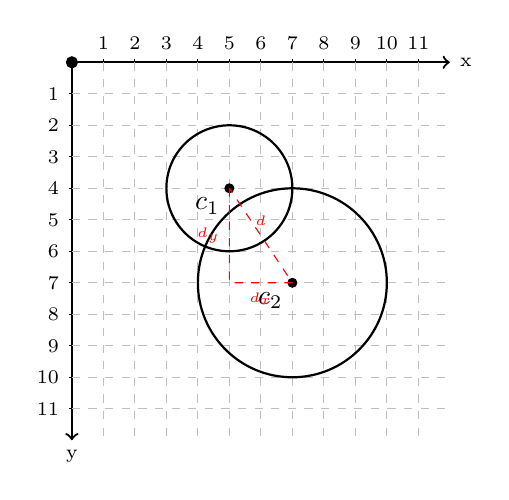
\begin{tikzpicture}
            \begin{scope}[yscale=-1, yshift=-5cm, xshift=5cm, scale=0.4]
                \drawaxesgrid{12}{12}
                % First circle
                \draw [black, thick] (5, 4) circle (2);
                % a point at the center of the first circle
                \filldraw [black] (5, 4) circle (4pt) node[anchor=north east] {$c_1$};
                % Second circle
                \draw [black, thick] (7, 7) circle (3);
                % a point at the center of the second circle
                \filldraw [black] (7, 7) circle (4pt) node[anchor=north east] {$c_2$};

                % Draw triangle representing dx, dy, d
                \draw [red, dashed] (5, 4) -- (5, 7) -- (7, 7) -- cycle;

                % Label dx, dy, d
                \node [red, anchor=east] at (5, 5.5) {\tiny $d_y$};
                \node [red, anchor=north] at (6, 7) {\tiny $d_x$};
                \node [red, anchor=south] at (6, 5.5) {\tiny $d$};

            \end{scope}
        \end{tikzpicture}
    \end{center}
    \columnbreak
    \begin{equation*}
        \begin{aligned}
            d_x           & = 7 - 5 = 2,                                      \\
            d_y           & = 7 - 4 = 3,                                      \\
            d             & = \sqrt{2^2 + 3^2} = \sqrt{13} \approx 3.61,      \\
            r_1 + r_2     & = 2 + 3 = 5,                                      \\
            d < r_1 + r_2 & \Rightarrow \text{Both circles are intersecting}. \\
                          & \therefore \text{Collision detected.}
        \end{aligned}
    \end{equation*}
\end{multicols*}

\begin{mdframed}[linecolor=black!30!white,linewidth=.5pt,extratopheight=3em]
    \begin{lstlisting}[language=C++, aboveskip=3mm,
        belowskip=3mm,
        showstringspaces=false,
        columns=flexible,
        basicstyle={\small\ttfamily},
        numbers=left,
        numberstyle=\tiny\color{gray},
        keywordstyle=\color{blue},
        commentstyle=\color{dkgreen},
        stringstyle=\color{mauve},
        breaklines=true,
        breakatwhitespace=true,
        tabsize=3,
        xleftmargin=1em]
#include "Vec2.h"
#include <cmath>
#include <iostream>

struct Circle {
    Vec2 center;
    float radius;
};

bool checkCollision(const Circle &c1, const Circle &c2) {
    const float dx = c2.center.x - c1.center.x;
    const float dy = c2.center.y - c1.center.y;
    const float distance = std::sqrt(dx * dx + dy * dy);
    const float sumOfRadii = c1.radius + c2.radius;
    const bool collision = distance < sumOfRadii;

    return collision;
}

int main() {
    Circle c1 = {{5, 4}, 2};
    Circle c2 = {{7, 7}, 3};

    if (checkCollision(c1, c2)) {
        std::cout << "Collision detected!" << std::endl;
    } else {
        std::cout << "No collision detected." << std::endl;
    }

    return 0;
}
\end{lstlisting}

\end{mdframed}

\begin{center}
    \textbf{Listing 1:} \textit{Collision Detection for Bounding Circles in C++}
\end{center}

\newpage

\subsection{Axis Aligned Bounding Boxes (AABB)}
In 2D games, objects are often enclosed in rectangles known as bounding boxes.
These are usually the smallest possible rectangle that completely encompasses
the texture's width and height. However, this is not always the case, as some
imperfections may exist such as the entity being larger than the bounding box.

Rectangles can be oriented in any direction as long as all four sides meet at
90-degree angles. This creates complexity in collision detection, requiring
calculations for line-line intersections. To simplify this, we can use
something called an axis-aligned bounding box (AABB). An AABB is a rectangle
that is aligned with the x and y axes, i.e. with sides parallel to the
coordinate axes.

\subsubsection{Point and AABB Intersection}

The simplest calculation for AABBs is to check whether a point is inside the
rectangle. Given a point $p$ and a rectangle with corners $c_1$ and $c_2$, we
can determine if the point is inside the rectangle by checking if the point's x
and y coordinates are within the rectangle's x and y coordinates. This is done
by the following formula:
\begin{center}
    \textit{Point $p$ is inside rectangle with corners $c_1$ and $c_2$ if and only if:} \\
    $(p.x > c_1.x) \land (p.x < c_2.x) \land (p.y > c_1.y) \land (p.y < c_2.y)$
\end{center}

If the rectangle is defined by a top left corner $c$, width $w$, and height
$h$, the equation can be modified to:

\begin{center}
    \textit{Point $p$ is inside rectangle with top left corner $c$, width $w$ and height $h$ if and only if:} \\
    $(p.x > c.x) \land (p.x < c.x + w) \land (p.y > c.y) \land (p.y < c.y + h)$
\end{center}
When broken down, the formula is evaluating four conditions:
\begin{multicols}{2}
    \begin{enumerate}
        \item The point's x-coordinate is to the right of the left side of the rectangle.
              \begin{equation*}
                  \begin{aligned}
                      p.x & > c_1.x \\
                      p.x & > c.x
                  \end{aligned}
              \end{equation*}

        \item The point's x-coordinate is to the left of the right side of the rectangle.
              \begin{equation*}
                  \begin{aligned}
                      p.x & < c_2.x   \\
                      p.x & < c.x + w
                  \end{aligned}
              \end{equation*}
    \end{enumerate}
\end{multicols}

\begin{multicols}{2}
    \begin{enumerate}
        \item[3.]The point's y-coordinate is above the bottom side of the rectangle.
        \begin{equation*}
            \begin{aligned}
                p.y & > c_1.y \\
                p.y & > c.y
            \end{aligned}
        \end{equation*}

        \item[4.] The point's y-coordinate is below the top side of the rectangle.
            \begin{equation*}
                \begin{aligned}
                    p.y & < c_2.y   \\
                    p.y & < c.y + h
                \end{aligned}
            \end{equation*}
    \end{enumerate}
\end{multicols}
\newpage
\begin{mdframed}[linecolor=black!30!white,linewidth=.5pt,extratopheight=1em]
    \begin{lstlisting}[language=C++, aboveskip=3mm,
        belowskip=3mm,
        showstringspaces=false,
        columns=flexible,
        basicstyle={\small\ttfamily},
        numbers=left,
        numberstyle=\tiny\color{gray},
        keywordstyle=\color{blue},
        commentstyle=\color{dkgreen},
        stringstyle=\color{mauve},
        breaklines=true,
        breakatwhitespace=true,
        tabsize=3,
        xleftmargin=1em]
#include "Vec2.h"
#include <iostream>

struct AABB {
    Vec2 topLeft;
    float width;
    float height;
};

bool pointInsideAABB(const Vec2 &p, const AABB &aabb) {
    const bool inside = p.x > aabb.topLeft.x &&
                        p.x < aabb.topLeft.x + aabb.width &&
                        p.y > aabb.topLeft.y &&
                        p.y < aabb.topLeft.y + aabb.height;

    return inside;
}
\end{lstlisting}

\end{mdframed}
\begin{center}
    \textbf{Listing 2:} \textit{Point Inside AABB in C++}
\end{center}

\newpage
\subsubsection{AABB Intersection}

Determining if two AABBs intersect is a relatively simple task. Given two
AABBs, one may be inclined to check for collision using the point inside AABB
method. However, this is not the most efficient method, as it requires checking
all four corners of one rectangle against the other rectangle. Instead, we can
use an algorithm that detects both horizontal and vertical overlap.

Given two AABBs with top left corners $c_1$ and $c_2$, we can determine if they
overlap horizontally by checking if the right side of the first rectangle is to
the right of the left side of the second rectangle and vice versa. This is done
by the following formula:

\begin{equation}
    \begin{aligned}
         & \textit{Rectangles overlap horizontally if and only if:} \\
         & (c_1.x < c_2.x + c_2.w) \land (c_1.x + c_1.w > c_2.x)
    \end{aligned}
\end{equation}

In a similar manner, we can determine if the rectangles overlap vertically by
checking if the top side of the first rectangle is above the bottom side of the
second rectangle and vice versa. This is done by the following formula:

\begin{equation}
    \begin{aligned}
         & \textit{Rectangles overlap vertically if and only if:} \\
         & (c_1.y < c_2.y + c_2.h) \land (c_1.y + c_1.h > c_2.y)
    \end{aligned}
\end{equation}

Put all together, the AABBs overlap if and only if they overlap both
horizontally and vertically. This is done by the following formula:

\begin{equation}
    % \begin{aligned}
    %      & [(c_1.x < c_2.x + c_2.w) \land (c_1.x + c_1.w > c_2.x)]      \\
    %      & \land[(c_1.y < c_2.y + c_2.h) \land (c_1.y + c_1.h > c_2.y)] \\
    % \end{aligned}
    \begin{aligned}
         & \hspace{1.1em} (c_1.x < c_2.x + c_2.w) \\
         & \land (c_1.x + c_1.w > c_2.x)          \\
         & \land (c_1.y < c_2.y + c_2.h)          \\
         & \land (c_1.y + c_1.h > c_2.y)
    \end{aligned}
\end{equation}

Example of AABB intersection:
\begin{center}
    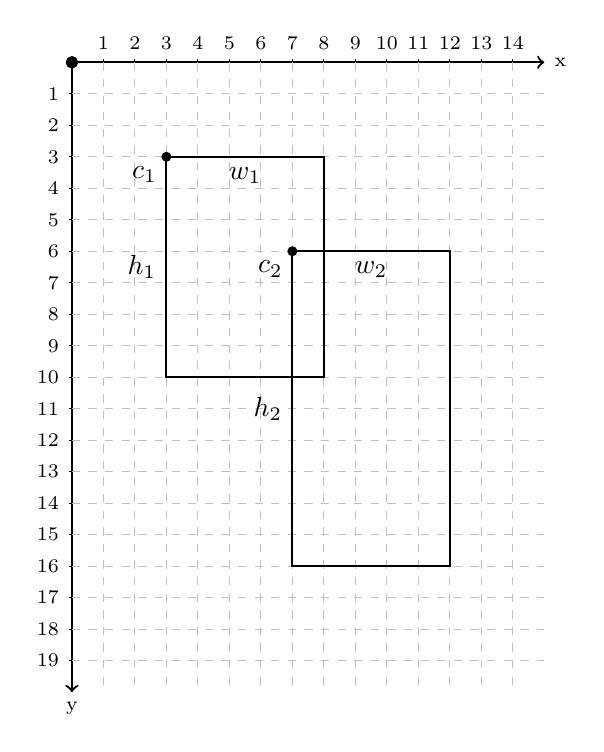
\begin{tikzpicture}
        \begin{scope}[yscale=-1, yshift=-5cm, xshift=5cm, scale=0.4]

            \drawaxesgrid{15}{20}

            % a point at the origin (0, 0) 
            \filldraw [black] (0, 0) circle (5pt) {};

            % First rectangle
            \draw [black, thick] (3, 3) rectangle (8, 10);
            \draw[black, thick, -] (3, 3) -- (8, 3) node[midway, below] {$w_1$};
            \draw[black, thick, -] (3, 3) -- (3, 10) node[midway, left] {$h_1$};
            % a point at the top left corner of the first rectangle

            \filldraw [black] (3, 3) circle (4pt) node[anchor=north east] {$c_1$};
            % Second rectangle
            \draw [black, thick] (7, 6) rectangle (12, 16);
            \draw[black, thick, -] (7, 6) -- (12, 6) node[midway, below] {$w_2$};
            \draw[black, thick, -] (7, 6) -- (7, 16) node[midway, left]
            {$h_2$};
            % a point at the top left corner of the second rectangle
            \filldraw [black] (7, 6) circle (4pt) node[anchor=north east] {$c_2$};

        \end{scope}
    \end{tikzpicture}
\end{center}

\begin{center}
    \textbf{Figure 1:} \textit{AABB Intersection Example}

\end{center}

It is important to note that the above formula can only check whether or nor
not two AABBs intersect. It does not provide information on how much they
intersect. To determine the overlap, we can use a calculation that takes a
center point and the width and height of the bounding box. This is done as
follows:

Given two AABBs with centers $c_1$ and $c_2$, widths $w_1$ and $w_2$, and
heights $h_1$ and $h_2$,

\begin{equation}
    \begin{aligned}
        \Delta                        & = \left\{ \left| c_1.x - c_2.x \right| , \left| c_1.y - c_2.y \right| \right\}                                                                                     \\
        O                             & = \left\{ \left[ \left( \frac{w_1}{2} + \frac{w_2}{2} \right) - \Delta_x \right] , \left[ \left( \frac{h_1}{2} + \frac{h_2}{2} \right) - \Delta_y \right] \right\} \\
        ( O_x > 0 ) \land ( O_y > 0 ) & \rightarrow \text{AABBs intersect}
    \end{aligned}
\end{equation}

In this formula, the vector $\Delta$ represents the absolute difference between
the center coordinates of the two AABBs along the $x$ and $y$ axes.

The vector $O$ represents the overlap between the two AABBs along the $x$ and
$y$ axes. The overlap along each axis is calculated by subtracting the
difference between the centers from the sum of the half-widths (for the $x$
axis) or half heights (for the $y$ axis) of the two AABBs. Here is an
implementation of the AABB intersection algorithm in C++:

\begin{mdframed}[linecolor=black!30!white,linewidth=.5pt,extratopheight=1em]
    \begin{lstlisting}[language=C++, aboveskip=3mm,
        belowskip=3mm,
        showstringspaces=false,
        columns=flexible,
        basicstyle={\small\ttfamily},
        numbers=left,
        numberstyle=\tiny\color{gray},
        keywordstyle=\color{blue},
        commentstyle=\color{dkgreen},
        stringstyle=\color{mauve},
        breaklines=true,
        breakatwhitespace=true,
        tabsize=3,
        xleftmargin=1em]

#include "Vec2.h"
#include <iostream>

struct AABB {
    Vec2 center;
    float width;
    float height;
};

bool checkAABBIntersection(const AABB &a, const AABB &b) {
    const Vec2 delta = {
        std::abs(a.center.x - b.center.x), 
        std::abs(a.center.y - b.center.y)
    };

    const Vec2 overlap = {
        (a.width / 2 + b.width / 2) - delta.x,
        (a.height / 2 + b.height / 2) - delta.y
    };
    
    const bool AABBIntersects = overlap.x > 0 && overlap.y > 0;

    return AABBIntersects;
}

\end{lstlisting}
\end{mdframed}

% \begin{mdframed}[linecolor=black!30!white,linewidth=.5pt,extratopheight=1em]
%     \begin{lstlisting}[language=C++, aboveskip=3mm,
%         belowskip=3mm,
%         showstringspaces=false,
%         columns=flexible,
%         basicstyle={\small\ttfamily},
%         numbers=left,
%         numberstyle=\tiny\color{gray},
%         keywordstyle=\color{blue},
%         commentstyle=\color{dkgreen},
%         stringstyle=\color{mauve},
%         breaklines=true,
%         breakatwhitespace=true,
%         tabsize=3,
%         xleftmargin=1em]
% #include "Vec2.h"
% class CTransform : public Component {
%     public :
%         Vec2 position = {0, 0};
%         Vec2 previousPosition = {0, 0};
%         Vec2 scale = {1.0, 1.0};
%         float angle = 0;
% };

% class CBoundingBox : public Component {
%     public :
%         Vec2 size;
%         Vec2 halfSize;
%         CBoundingBox(const Vec2 &size) : size(size), halfSize(size / 2) {}
% };

%         \end{lstlisting}
% \end{mdframed}

\newpage
\section*{Appendix}
\subsection*{Vec2.h}
\vspace{1em}
\begin{mdframed}[linecolor=black!30!white,linewidth=.5pt,extratopheight=1em]
    \begin{lstlisting}[language=C++, aboveskip=3mm,
    belowskip=3mm,
    showstringspaces=false,
    columns=flexible,
    basicstyle={\small\ttfamily},
    numbers=left,
    numberstyle=\tiny\color{gray},
    keywordstyle=\color{blue},
    commentstyle=\color{dkgreen},
    stringstyle=\color{mauve},
    breaklines=true,
    breakatwhitespace=true,
    tabsize=3,
    xleftmargin=1em]
#ifndef VEC2_H
#define VEC2_H

class Vec2 {
public:
};
    double x, y;

    Vec2(float x = 0, float y = 0);

    bool operator==(const Vec2 &rhs) const;
    bool operator!=(const Vec2 &rhs) const;

    Vec2 operator-(const Vec2 &rhs) const;
    Vec2 operator+(const Vec2 &rhs) const;
    Vec2 operator*(const float val) const;
    Vec2 operator/(const float val) const;

    void operator+=(const Vec2 &rhs);
    void operator-=(const Vec2 &rhs);
    void operator*=(const float val);
    void operator/=(const float val);

    Vec2  normalize();
    float length() const;
};

#endif // VEC2_H
\end{lstlisting}
\end{mdframed}
\end{document}
